\section{Einleitung}
\label{sec1:intro}
Die Digitalisierung der Welt schreitet immer rasanter voran. Nicht zuletzt wird im Kontext der Digitialisierung auch von dem \enquote{Informationszeitalter} und \enquote{Computerisierung} gesprochen \cite{gabler-digitalisierung}.
In einer zunehmend digitaleren Welt nimmt die Anzahl der digitalen Geräten und Anwendern derselben immer mehr zu.
Laut Statistiken belief sich die Zahl der Internetnutzer, den sogenannten Onlinern, im Jahr 2022 auf rund 5.3 Milliarden. 
Im Vergleich zum letzten Jahrzehnt ist somit die Anzahl der Internetanwender innerhalb eines Jahrzehnts um rund 2.9 Milliarden auf beinahe das Doppelte angestiegen \cite{statista-onliner-2022}.
Auch die weltweite Covid-19 Pandemie 20/21 hatte keinen hindernden Effekt auf diese Entwicklung.
Im Gegenteil.
Aufgrund von Lockdowns verbrachten viele Menschen Zeit zu Hause und wandten sich vermehrt den sozialen Medien zu, um mit Freunden und Bekannten in Kontakt zu bleiben \cite{statista-covid-social-media-use}.
Die Verwendung von sozialen Medien, wie Instagram, Facebook, Snapchat und weiteren führt zu enormen Datenmengen, die ohne Hilfsmittel für Menschen nicht mehr greifbar und überschaubar sind.
\med
Soziale Medien sind allerdings nicht der einzige Anwendungsbereich, in welchem gewaltige Datenmengen anfallen.
So ist ein anderer Anwendungsbereich z.B. die Medizin bzw. das Gesundheitswesen.
Ein konkretes und aktuelles Beispiel liegt z.B. in den angefallen Daten von sogenannten \textit{Smart Wearables}. 
\textit{Smart Wearables} sind kleine elektronische Systeme, die u.a. in Alltagsgegenständen oder am oder gar im Körper getragen werden können.
Konkretere Beispiele sind Smartwatches, Fitnesstracker, Blutdruckmessgeräte oder Biosensoren (siehe \cref{sec1:intro:fig:smart-watch}).
Diese Systeme können zu medizinischen Zwecken verwendet werden und sammeln kontinuierlich Daten vom Träger bzw. Anwender.
\par
\begin{figure}[htb]
    \centering
    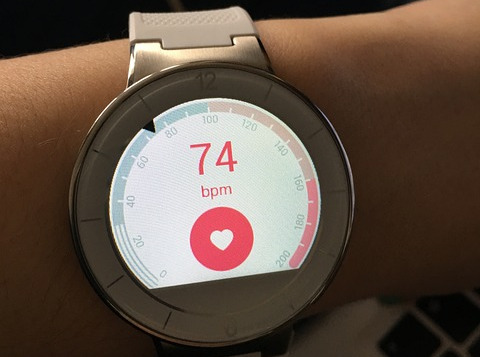
\includegraphics[width=5cm]{resources/images/smartwatch.jpg}
    \caption{Smartwatch mit Herzschläge pro Minute.}
    \label{sec1:intro:fig:smart-watch}
\end{figure}
\noindent
Sollen, unabhängig vom Anwendungsbereich, diese angefallenen Daten und daraus extrahierten Merkmale effektiv verarbeitet und gewonnene Erkenntnisse effektiv kommuniziert werden, so muss die semantische Lücke zwischen den identifizierten Merkmalen und einer geeigneten semantischen Darstellung überbrückt werden.
Eine geeignete semantische Darstellung bezeichnet hierbei eine für Menschen lesbare und verständliche Erklärung.
Das Überbrücken dieser semantischen Lücke wird seit Jahren intensiv erforscht und ist Gegenstand zahlreicher Untersuchungen im Bereich des \mmiri{}.
In dieser Arbeit wird untersucht, ob und inwiefern generative künstliche Intelligenz (KI) verwendet werden kann, um die semantische Lücke zu schließen und inwieweit generative KI geeignet ist, präzise Erklärungen aus identifizierten Merkmalen zu generieren.

\subsection{Motivation}
\label{sec1:intro:subsec:motivation}
Bei dieser Arbeit handelt es sich um eine Bachelorarbeit am Lehrgebiet Multimedia und Internetanwendungen (MMIA) von Prof. Dr-Ing. Matthias Hemmje. 
Schon vor der Bachelorarbeit bin ich über das von diesem Lehrgebiet angebotene Fachpraktikum Multimedia Information Retrieval mit dem Bereich \mmir{} in Kontakt gekommen. 
Da mich das Fachpraktikum und das Themengebiet des \mmir{} sehr interessiert und begeistert hat, schreibe ich nun in diesem Lehrgebiet meine Bachelorarbeit, um meine Fähigkeiten auszubauen und mein Wissen zu vertiefen.
\med
Das Thema dieser Arbeit ist im Bereich \mmir{} und künstlicher Intelligenz verortet. 
Das Themengebiet der künstlichen Intelligenz ist nicht neu und schon seit Jahrzehnten Gegenstand der Forschung und zahlreicher Untersuchungen. 
Die Anwendungsmöglichkeiten von künstlicher Intelligenz sind weitreichend und haben zunehmend Einfluss auf unseren Alltag. 
Viele Aufgaben, die früher von Menschen erledigt wurden, oder nicht zu erledigen waren, werden bereits durch künstliche Intelligenz übernommen und automatisiert. 
Weiterhin stellt künstliche Intelligenz für viele Unternehmen und Organisationen schon heute effektiv einen wirtschaftlichen Mehrwert dar. 
Aus diesen Gründen ist dieses Thema auch persönlich für mich von Interesse.
\med
Das Lehrgebiet MMIA hat zum Zwecke der Forschung im Bereich des \mmir{} das Forschungsprojekt \gmafi{} ins Leben gerufen. 
Dieses Forschungsprojekt wurde entwickelt, um aktuelle Missstände und Probleme des einfachen \mmir{} auf intelligente Art und Weise zu adressieren. 
Das \gmaf{} hat dabei zum Ziel durch eine intelligente Erweiterung von \mmir{} semantische, erklärbare, für Menschen verständliche, effektive, effiziente, kompatible und integrierte Lösungen anzubieten \cite[S.~20]{swa_diss}. 
Diese Erweiterung wird \smmiri{} genannt. 
\smmir{} führt eine Reihe von Konzepten ein, die über klassisches \mmir{} hinaus gehen. 
Hierzu gehören erweiterte Metriken für die Berechnung von Ähnlichkeit oder Empfehlungen, Möglichkeiten der Merkmalsintegration und -fusion, sowie die Erklärbarkeit von \mmir{}-Prozessen und deren Inhalte.
\par
\begin{figure}[htb]
    \centering
    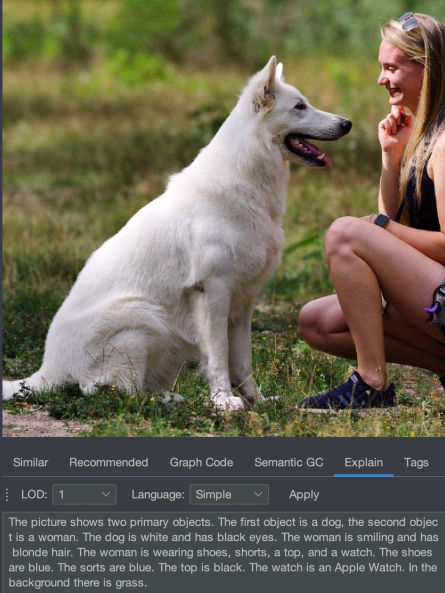
\includegraphics[width=0.8\textwidth]{resources/images/gmaf-explain-ui-dog-man-example.png}
    \caption{Beispiel für eine generierte textuelle Beschreibung eines Bildes im \gmaf{}.}
    \label{sec1:intro:subsec:motivation:fig:gmaf-explain-ui-dog-man-example}
\end{figure}
\noindent
Unter Erklärbarkeit versteht man in diesem Zusammenhang für Menschen verständliche Antworten auf Fragestellungen, wie z.B. die Frage \enquote{Was ist die wichtigste Eigenschaft des Elements?} oder \enquote{Was ist der Unterschied zwischen diesen zwei Bildern?}.
Sollen Antworten auf diese Fragen auf für Menschen verständliche Art und Weise ausgedrückt werden, so müssen diese Antworten auf natürlicher Sprache aufbauen, oder prägnant visuell dargestellt werden.
Das \gmaf{} bietet bereits diverse Implementierungen zur Generierung von textuellen Beschreibungen von \mmir{}-Inhalten in für Menschen lesbarer und verständlicher Form. 
Ein Beispiel für so eine generierte textuelle Erklärung ist in \cref{sec1:intro:subsec:motivation:fig:gmaf-explain-ui-dog-man-example} zu sehen.
Die in \cref{sec1:intro:subsec:motivation:fig:gmaf-explain-ui-dog-man-example} gezeigte Benutzungsschnittstelle bietet die Möglichkeit, die anhand der identifizierten Merkmale generierte Erklärung anzupassen. 
So lässt sich z.B. die Komplexität der Sprache anpassen. 
Genauer kann hier zwischen einfacher, normaler und komplexer Sprache gewählt werden.



Trotz der komplex gewählten Sprache sind die Sätze in der Erklärung nur sehr rudimentär und weisen keine hohe Komplexität auf.
Zum Zeitpunkt des Verfassens dieser Arbeit bietet das \gmaf{} keine Implementierung, die präzise textuelle Beschreibungen generieren kann.
Das Generieren von präzisen textuellen Beschreibungen anhand identifizierter Merkmale stellt somit eine noch offene Forschungslücke dar. 
Eine weitere Forschungslücke ist, dass das \gmaf{} keine Möglichkeiten bereitstellt Erklärungen in anderweitiger Form, so z.B. in einer visuellen Form zu generieren und zu präsentieren.
Aufgrund der immer wachsenden Datenmengen und der damit einhergehenden Unüberschaubarkeit sind präzisere Erklärungen von Merkmalen dieser Datenmengen für Benutzer sehr hilfreich und können, je nach Anwendungsfall, einen echten und signifikanten Mehrwert für diese darstellen.

\clearpage

\subsection{Problembeschreibung}
\label{sec1:intro:subsec:problems}

\clearpage

\subsection{Forschungsfragen}
\label{sec1:intro:subsec:research-questions}

{
    \def\arraystretch{1.1}%
    \begin{xltabular}{\linewidth}{
            @{}
            >{
                \hsize=0.15\linewidth
                \raggedright\arraybackslash
            }X
            >{
                \hsize=0.75\linewidth
                \raggedright\arraybackslash
            }X
            >{
                \hsize=0.1\linewidth
                \centering\arraybackslash
            }X
            @{}
    }

    % First Header

    \caption{Aufschlüsselung der Forschungsfragen auf Forschungsziele} 
    \label{sec1:intro:table:research-questions} \\
        
    \toprule
    \multicolumn{3}{
        >{
            \hsize=\linewidth\centering\arraybackslash
        }X
    }
    {
        \textbf{Forschungsfragen}
    } \\ 
    \midrule
         
    \textbf{FZ} & \multicolumn{1}{c}{\textbf{Beschreibung}} & \textbf{PB} \\ 
    \midrule
    
    \endfirsthead

    % Normal Head

    \toprule
    \multicolumn{3}{
        >{
            \hsize=\linewidth\centering\arraybackslash
        }X
    }
    {
        \textbf{Forschungsfragen}
    } \\ 
    \midrule
         
    \textbf{FZ} & \multicolumn{1}{c}{\textbf{Beschreibung}} & \textbf{PB} \\ 
    \midrule
    
    \endhead
        
    % Lower Rows

    \multicolumn{3}{
        >{
            \hsize=\linewidth\centering\arraybackslash
        }X
    }
    {
        \textbf{Erklärbarkeit von MMIR mittels generativer KI}
    } \\ \midrule

    FZ 1.1/O 
    & 
    Recherche zur Erklärbarkeit von MMIR mittels generativer KI
    & PB1 \\

    \midrule

    FZ 1.2/TB 
    & 
    Modellierung zur Erklärbarkeit von MMIR mittels generativer KI
    & PB1 \\

    \midrule

    FZ 1.3/I
    & 
    Implementierung zur Erklärbarkeit von MMIR mittels generativer KI
    & PB1 \\

    \midrule

    FZ 1.4/E 
    & 
    Experiment zur Erklärbarkeit von MMIR mittels generativer KI
    & PB1 \\

    \midrule

    \multicolumn{3}{
        >{
            \hsize=\linewidth\centering\arraybackslash
        }X
    }
    {
        \textbf{Integration generativer KI in das GMAF}
    } \\ \midrule

    FZ 2.1/O 
    & 
    Recherche zur Integration generativer KI in das GMAF
    & PB2 \\

    \midrule

    FZ 2.2/TB 
    & 
    Modellierung zur Integration generativer KI in das GMAF
    & PB2 \\

    \midrule

    FZ 2.3/I
    & 
    Implementierung zur Integration generativer KI in das GMAF
    & PB2 \\

    \midrule

    FZ 2.4/E 
    & 
    Experiment zur Integration generativer KI in das GMAF
    & PB2 \\
        
    \bottomrule 

    \end{xltabular}
}

\clearpage

\subsection{Methodik und Ziele}
\label{sec1:intro:subsec:methodology-goals}
Um die im vorigen \cref{sec1:intro:subsec:research-questions} formulierten Forschungsfragen strukturiert beantworten zu können, wird diese Arbeit auf der vielfach bewährten Methodik von Nunamaker \cite{nunamaker} aufbauen. Die Methodik nach Nunamaker teilt ein zu lösendes Problem anhand von Recherche und Entwicklung in vier Phasen der Problemlösung auf. Diese vier Phasen lauten:
\begin{enumerate}
    \setlength{\itemsep}{0pt}
    \item Beobachtungsphase
    \item Theoriebildungsphase
    \item Systementwicklungs - bzw. Implementierungsphase
    \item Experimentphase
\end{enumerate}
\begin{figure}[htb]
    \centering
    \resizebox*{0.75\textwidth}{!}{
        \begin{minipage}{\textwidth}
            \begin{tcolorbox}[
                enhanced, width=\textwidth, height=\textwidth, colback=white, colframe=black,
                overlay={
                    \tikzset{
                        exstyle/.style={-{Triangle[angle=90:6pt,length=3mm,fill=black]}}
                    }
                    \def\rad{\textwidth-2.5cm}
                    \node [circle, minimum size=\rad] (c) at ([yshift=-0.8cm]frame.center) {};
                    \def\labellist{
                          \shortstack{
                            \Large \textbf{Beobachtung} \\
                            \rule{3cm}{1pt} \\
                            \footnotesize
                            Umfragestudien, \\ 
                            \footnotesize
                            Fallstudien, \\
                            \footnotesize
                            Feldforschung
                          }, 
                          \shortstack{
                            \Large \textbf{Experiment} \\
                            \rule{3cm}{1pt} \\
                            \footnotesize
                            Computersimulationen,\\ 
                            \footnotesize
                            Feldexperimente, \\
                            \footnotesize
                            Laborexperimente
                          },
                          \shortstack{
                            \Large \textbf{Theorie} \\ \Large \textbf{Bildung} \\
                            \rule{3cm}{1pt} \\
                            \footnotesize
                            konzept. Rahmen-\\ 
                            \footnotesize
                            bedingungen, mathe\\
                            \footnotesize
                            matische Modelle\\
                            \footnotesize 
                            Methoden
                          }
                    }
                    
                    \foreach [count=\i] \x in \labellist {
                        
                        \node (n\i) [draw, fill=white, minimum size=0cm, inner sep=0mm, circle] at (c.\i*360/3+90) {
                            \scalebox{0.8}{
                                \x
                            }
                        };
                    }
                    \node (nm) [draw, fill=white, minimum size=0cm, inner sep=0mm, circle] at (c.center) {
                        \scalebox{0.8}{
                            \shortstack{
                                \Large \textbf{System} \\ \Large \textbf{Entwicklung} \\
                                \rule{3cm}{1pt} \\
                                \footnotesize
                                Produktentwicklung,\\ 
                                \footnotesize
                                Technologietransfer, \\
                                \footnotesize
                                Prototyping
                            }
                        }
                    };
                    \node [anchor=south east, rectangle, minimum width=4cm, rounded corners, text=white, fill=black, inner sep=1.7mm] at (frame.south east) {
                        \textbf{nach J. Nunamaker}
                    };

                    \draw[exstyle] (nm.200) -- (n1.40);
                    \draw[exstyle] (n1.25) -- (nm.215);

                    \draw[exstyle] (nm.340) -- (n2.140);
                    \draw[exstyle] (n2.155) -- (nm.325);

                    \draw[exstyle] (nm.{83}) -- (n3.{277});
                    \draw[exstyle] (n3.{263}) -- (nm.{97});

                    \draw[exstyle, bend left=41.5](n3.0) to (n2.60);
                    \draw[exstyle, bend left=41.5](n2.240) to (n1.300);
                    \draw[exstyle, bend left=41.5](n1.120) to (n3.180);

                    \draw[exstyle, bend right=41.5](n2.78) to (n3.342);
                    \draw[exstyle, bend right=41.5](n1.318) to (n2.222);
                    \draw[exstyle, bend right=41.5](n3.198) to (n1.102);

                    \node[circle, fill=white, draw, minimum size=1cm] at (n1.71) {1};
                    \node[circle, fill=white, draw, minimum size=1cm] at (n3.25) {2};
                    \node[circle, fill=white, draw, minimum size=1cm] at (nm.45) {3};
                    \node[circle, fill=white, draw, minimum size=1cm] at (n2.110) {4};
                }
            ]
            \end{tcolorbox}
        \end{minipage}
    }
    \caption{Phasen der Problemlösung nach Nunamaker \cite{nunamaker}.}
    \label{sec1:intro:subsec:methodology-goals:fig:nunamaker}
\end{figure}
In der Beobachtungsphase werden im Rahmen einer Recherche Informationen gesammelt. 
In der Theoriebildungsphase werden Konzepte für Lösungen konzipiert und modelliert. 
Die Systementwicklungs bzw. Implementierungsphase beschäftigt sich mit der Entwicklung von Lösungen basierend auf den Theorien aus der Theoriebildungphase bzw. Beobachtungen aus der Beobachtungsphase, und welche in der letzten Phase, der Experimentphase evaluiert werden können. 
Diese Phasen sind eng miteinander verwoben und jede Phase mündet mit seinem Ergebnis in den anderen Phasen und trägt zu diesen bei. 
Durch die Methodik von Nunamaker wird sichergestellt, dass jedes Forschungsziel eindeutig einer Problembeschreibung zugeordnet werden kann.

\subsection{Ansatz auf Aufbau der Arbeit}
\label{sec1:intro:subsec:approach-structure}
Die Struktur dieser Arbeit ergibt sich 1:1 aus der Methodik von Nunamaker. Dadurch wird sichergestellt, dass jede Forschungsfrage in dieser Arbeit abgearbeitet wird. Im Folgenden werden die einzelnen Forschunsziele ihren Phasen nach in die jeweiligen Kapitel umgruppiert.
\begin{itemize}
    \setlength{\itemsep}{0pt}
    \item \textbf{\enquote{Kapitel 2 - Stand der Wissenschaft und Technik}} deckt alle Forschungsziele vom Typ \textit{Beobachtung} ab, und wird der Reihenfolge nach den aktuellen Stand der Wissenschaft und Technik zusammenfassen, einführen und darstellen.
    \item \textbf{\enquote{Kapitel 3 - Modellierung}} deckt alle Forschungsziele vom Typ \textit{Theoriebildung} ab und beschreibt die Modellierung und das Design von Konzepten und Algorithmen zu vorgeschlagenen Problemlösungen.
    \item \textbf{\enquote{Kapitel 4 - Implementierung}} beschreibt die Implementierung von Modellen und Konzepten und deckt alle Forschungsziele vom Typ \textit{Systementwicklung bzw. Implementierung}.
    \item \textbf{\enquote{Kapitel 5 - Experiment}} deckt alle Forschungsziele vom Typ \textit{Experiment} ab und gibt eine detaillierte Beschreibung aller Ergebnisse.
\end{itemize}
Daraus ergibt sich, dass die Unterkapitel in einer 1:1 Korrespondenz zu jeweiligen Forschungszielen stehen. Eine vorläufige Gliederung des späteren Dokuments ergibt sich folglich automatisch.

\subsection{Arbeits- und Zeitplan}
\label{sec1:intro:subsec:work-time-plan}